\section{Sviluppo}
\subsection{Sviluppo algoritmo per ricomposizione delle labels in un'immagine frammentata}
Al fine di implementare l'algoritmo è stata creata una libreria contenente numerose funzioni per lavorare con le labels ritornate dal modello che esegue la detection. Ad esempio è possibile ottenere la posizione delle bounding boxes o controllare le loro intersezioni con altre entità e calcolarne l'IoU. Una labels è composta da un array di tipo numpy formato da quattro numeri interi caratterizzanti le coordinate del vertice in alto a sinistra e quello in basso a destra del bounding box, un intero per rappresentare la categoria di appartenenza dell'elemento ed infine un numero decimale compreso tra 1 e 0 per indicarne lo score.\\
Al fine di rendere l'algoritmo più flessibile viene data la possibilità ad un utente di ridefinire alcune funzioni in modo da adattarle alle proprie esigenze adottando un design pattern di tipo template. In particolare le funzioni ridefinibili sono la \textbf{condizione di correlazione}, la \textbf{regola di classificazione} più una terza funzione che è in grado di, dato in input un gruppo di bounding boxes, ritornare come output la bounding box risultante dalla loro unione. Tutte e tre le funzioni ridefinite possono essere passate come direttamente tra i parametri dell'algoritmo, altrimenti verranno utilizzate alcune funzioni di default il cui comportamento è quello descritto nella sezione \textit{4.1}.\\
Altri parametri passabili includono: una lista di labels trovate con una detection ed eventualmente pre-processate con NMS, le dimensioni delle regioni, dello stride e della quantità di overlap, sia in verticale che in orizzontale, il valore della tolleranza in pixels ed il valore della soglia di matching in percentuale.
Alla fine l'algoritmo ritornerà una lista di tutte le labels presenti nell'immagine dopo l'elaborazione.\\ Nella seguente sezione ne viene riportata una sua possibile implementazione.
\subsubsection{Implementazione}
\begin{lstlisting}[language=Python, caption=Python example]
import numpy as np
import modules.labels as lb

def process_image_labels(boxes, region_size=(300, 300), stride_size=(300, 300), overlap=(0, 0), tol=0, threshold_match=50, group_condition=None, find_category=None, find_group_label=None):

    # set default functions
    if group_condition is None:
        group_condition = lb.group_condition
    if find_category is None:
        find_category = lb.find_category
    if find_group_label is None:
        find_group_label = lb.find_group_label

    w, h = lb.get_img_dim_from_boxes(boxes)
    regions = lb.generate_regions(w, h, region_size, stride_size)
    # Keeps only the labels intersecting one or more region edges
    ne_boxes, ne_boxes_indexes = lb.get_intersect_edge_labels(boxes, regions, tol, overlap)
    # All labels are set as not-checked and not-grouped
    checked = np.zeros((np.ma.size(ne_boxes, 0)))
    grouped = np.ones((np.ma.size(ne_boxes, 0))) * (-1)
    # number of label groups
    n_group = 0
    for i in range(len(ne_boxes)):
        checked_boxes = np.zeros((0, 6))
        # Select a label and sets it as checked
        if not checked[i]:
            checked[i] = True
            checked_boxes = np.vstack([checked_boxes, ne_boxes[i]])
            while True:
                found = 0
                # For each label checked but not-grouped:
                for j in range(len(ne_boxes)):
                    if checked[j] and grouped[j] == -1:
                        for k in range(len(ne_boxes)):
                            if not checked[k] and lb.intersection(ne_boxes[j], ne_boxes[k], tol) and group_condition(ne_boxes[j], ne_boxes[k]) and lb.intersect_common_edge(ne_boxes[j], ne_boxes[k], regions, tol, overlap) and lb.matched(ne_boxes[j], ne_boxes[k], threshold_match) and not lb.belong_same_region_strict_group(ne_boxes[k], checked_boxes, regions, 0):
                                # The new label is set as checked
                                checked[k] = True
                                found += 1
                                checked_boxes = np.vstack([checked_boxes, ne_boxes[k]])
                # The cycle is repeated until no new labels can be found
                if found == 0:
                    break
            # All the checked labels are set as grouped and is them assigned a number with the purpose to identify their group ID
            for j in range(len(ne_boxes)):
                if checked[j] and grouped[j] == -1:
                    grouped[j] = n_group
            n_group += 1

    # Now that we have grouped the labels, each group is merged into a label containing all of them
    new_boxes = np.zeros((0, 6))
    for i in range(n_group):
        v = np.zeros((0, 6))
        for j in range(len(ne_boxes)):
            if grouped[j] == i:
                v = np.vstack((v, ne_boxes[j]))
        # Find the coordinates of the label containing the whole group
        (xx1, yy1), (xx2, yy2) = find_group_label(v)
        # Find the category and the score of the label containing the whole group
        categories, scores = find_category(v)
        for j in range(len(categories)):
            new_boxes = np.vstack((new_boxes, np.array([xx1, yy1, xx2, yy2, categories[j], scores[j]])))
    # new_boxes are the labels resulting from grouping algorithm

    # The algorithm is over now thus we can return the results
    ne_boxes_indexes = ne_boxes_indexes.astype(int)
    old_boxes = np.delete(boxes, ne_boxes_indexes, 0)
    final_boxes = np.append(new_boxes, old_boxes, 0)

    return final_boxes
\end{lstlisting}
\subsubsection{Test di integrazione}
Al fine di verificarne la correttezza sono stati implementati 80 test di integrazione. Essi hanno il compito di testare l'algoritmo su diverse disposizioni e quantità di labels impostando i parametri con differenti valori in modo tale da riconoscerne il maggior numero di errori possibile. Sono state testate in totale cinque disposizioni di labels differenti con due diversi valori di overlap, tolleranza, stride e dimensione delle regioni arrivando ad un totale 80 test passati tutti con esito positivo.
\subsubsection{Pipeline completa}
L'algoritmo appena descritto è solo uno degli step che compongono la pipeline per eseguire la detection completa e poi poterla testare. Il procedimento completo viene descritto nella lista sottostante:
\begin{enumerate}
\item Detection;
\item NMS;
\item Inizializzazione parametri (opzionale);
\item Ricostruzione labels;
\item Calcolo metriche (opzionale).
\end{enumerate}
La detection viene effettuata tramite un modello già allenato messo a disposizione dall'azienda ed implementato con Tensorflow. In fase di implementazione sono state invece utilizzate una Faster-RCNN o una SSD (Single Shot MultiBox) allenate sul dataset Coco ed implementate in OpenCV. In particolare, l'elevata efficienza di SSD si è rivelata molto utile in caso servisse una detection molto veloce sacrificando però la qualità.\\
Successivamente, viene applicato l'algoritmo di NMS con la variante ANMS descritta nella sezione \textit{4.1} ai fini di garantire risultati migliori.\\
In fase di testing si potrebbe voler testare l'algoritmo di ricostruzione delle labels impostando diverse combinazioni di parametri in modo da selezionare quelli ottimali. Quest'operazione può essere portata a termine lanciando uno script bash in grado di eseguire diverse volte l'algoritmo sulla base di alcuni parametri impostati a piacere utilizzando sempre come input le labels ottenute da NMS. Al termine di ogni esecuzione, i risultati ottenuti vengono salvati sotto forma di file di testo e possono essere passati come input ad uno script in Python in grado di calcolare i valori delle metriche finali. I risultati sono stati salvati nel seguente formato per renderlo compatibile con lo script per calcolare le metriche:
\begin{enumerate}
\item \textbf{bbox\_left}: la coordinata x del vertice in alto a sinistra della bounding box predetta;
\item \textbf{bbox\_top}: la coordinata y del vertice in alto a sinistra della bounding box predetta;
\item \textbf{bbox\_right}: la coordinata x del vertice in basso a destra della bounding box predetta;
\item \textbf{bbox\_down}: la coordinata y del vertice in basso a destra della bounding box predetta;
\item \textbf{score}: affidabilità della predizione;
\item \textbf{object\_category}: categoria di appartenenza dell'oggetto predetto.
\end{enumerate}
I risultati ottenuti dalla pipeline completa verranno mostrati più avanti in sezione \textit{7} insieme ad una spiegazione dettagliata delle metriche utilizzate.

\newpage
\subsection{Sviluppo sistema di tracking}
Lo sviluppo del sistema di tracking su video è più complesso rispetto rispetto a quello dell'algoritmo di ricostruzione delle labels perciò ne verrà solamente riportato un diagramma delle classi in UML. E' da sottolineare che il diagramma non è completo ma ne è stata riportata una sua semplificazione.
\begin{figure}[H]
	\centering
	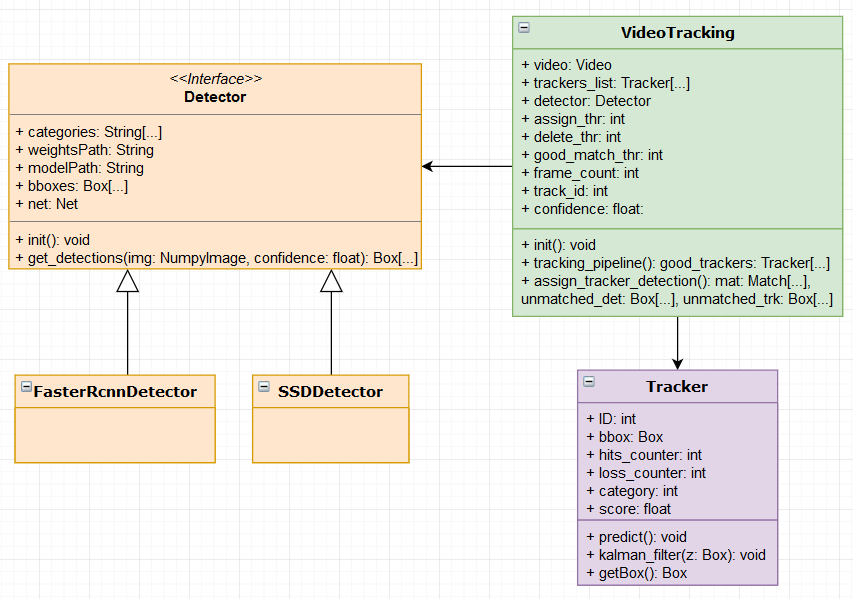
\includegraphics[width=0.9\linewidth]{images/diagramma-classi-tracking.png}
	\caption{Diagramma delle classi del sistema di tracking}
	\label{Diagramma delle classi del sistema di tracking}
\end{figure}
Nel diagramma si può individuare uno strategy pattern tra l'interfaccia \textit{Detector} e le sue due implementazioni \textit{FasterRcnnDetector} ed \textit{SSDDetector}. In questo modo, nel caso in cui servisse una nuova tipologia di rete per effettuare la detection, basta semplicemente implementare l'interfaccia \textit{Detector} con la struttura della nuova rete a patto che quest'ultima sia già stata sufficientemente allenata. Infatti, i campi dati \textit{weightsPath} e \textit{modelPath} indicano i percorsi dover trovare i files da cui leggere i pesi e la struttura del relativo modello. Il metodo che effettua la detection vera e propria è il metodo \textit{get\_detections}, il quale, data in input un'immagine in formato numpy ed una soglia di affidabilità ritorna una lista di labels sotto forma di numpy array corrispondenti agli elementi individuati.\\
La classe \textit{Tracker} implementa la tipologia di tracker descritta in sezione \textit{4.2}. Ogni tracker traccia un solo elemento tenendo quindi traccia del suo ID, la sua bounding box, la sua categoria ed il suo score. I campi dati \textit{hits\_counter} e \textit{loss\_counter} sono i rispettivi contatori di corrette associazioni in frames consecutivi e mancate associazioni sempre in frames consecutivi. I restanti metodi servono per interagire con il filtro di Kalman, in particolare il metodo \textit{kalman\_filter} si occupa della fase di aggiornamento mentre il metodo \textit{predict} svolge la fase di predizione.\\
La parte principale del sistema è formata dalla classe \textit{VideoTracking} la quale gestisce l'intera pipeline per svolgere il tracking. Ordinatamente, ogni frame del video viene processato dal metodo \textit{tracking\_pipeline}, il quale, ritorna i trackers corrispondenti alle labels da mostrare sul frame corrente. Per prima cosa viene richiamato il metodo \textit{assign\_tracker\_detection} che si occupa di effettuare le associazioni tracker-detection ed ottenere anche tutti i trackers e tutte le detections che per vari motivi non sono state assegnate. In seguito vengono aggiornati tutti i trackers con i relativi filtri e contatori, inoltre vengono creati dei nuovi trackers per tracciare gli eventuali nuovi elementi ed allo stesso tempo vengono cancellati quei trackers che da troppi frames consecutivi non sono stati associati. Infine la classe \textit{VideoTracking} completa l'iterazione mostrando a video le labels degli oggetti identificati e tracciati ed eventualmente salvando il frame appena elaborato in un cartella specifica in modo da poter ricostruire il video con il tracciamento applicato.\\
Anche in questo caso, come per la detection, è possibile salvare la lista degli oggetti tracciati sotto forma di file di testo. I risultati salvati rispettano il seguente formato:
\begin{enumerate}
\item \textbf{frame\_index}: indice del frame nel video;
\item \textbf{target\_id}: ID dell'oggetto;
\item \textbf{bbox\_left}: la coordinata x del vertice in alto a sinistra della bounding box predetta;
\item \textbf{bbox\_top}: la coordinata y del vertice in alto a sinistra della bounding box predetta;
\item \textbf{bbox\_width}: larghezza in pixels della bounding box predetta;
\item \textbf{bbox\_height}: altezza in pixels della bounding box predetta;
\item \textbf{score}: affidabilità della predizione;
\item \textbf{object\_category}: Categoria di appartenenza dell'oggetto predetto.
\end{enumerate}
Questo formato è lo stesso formato utilizzato dalla sfida VisDrone2019 in quanto lo script in Matlab utilizzato per calcolare le metriche finali e valutare la bontà del tracciamento è stato rilasciato pubblicamente dagli organizzatori stessi.

